\documentclass[main]{subfiles}

\begin{document}

\section{Eksperimentel Opstilling}
Delforsøg 1 og 2 har identisk opstilling på følgende punkter: En laser kilde pkt. 1 på \cref{fig:opstilling1} og \cref{fig:opstilling2} udsender en laser stråle på $\lambda_L =  \SI{911}{\nano\m} $. Herefter rammer laseren en linse, pkt. 2, der har til formål at danne en kollimeret laser stråle, hvorefter strålens føres over i AOM'en pkt. 5, via. 2 spejle pkt 3. og en linse pkt. 4, der fokusere laser strålen i AOM'ens indgang.

\subsection{Delforsøg 1}
I dette forsøg, er AOM'en forbundet til en frekvensgenerator og en forstærker ved hhv. pkt. $7$ og $8$ på \cref{fig:opstilling1}. Herefter bliver afstanden mellem laserstrålen diffraktionsordner målt på en skærm ved pkt. $6$.
\begin{figure}[H]
    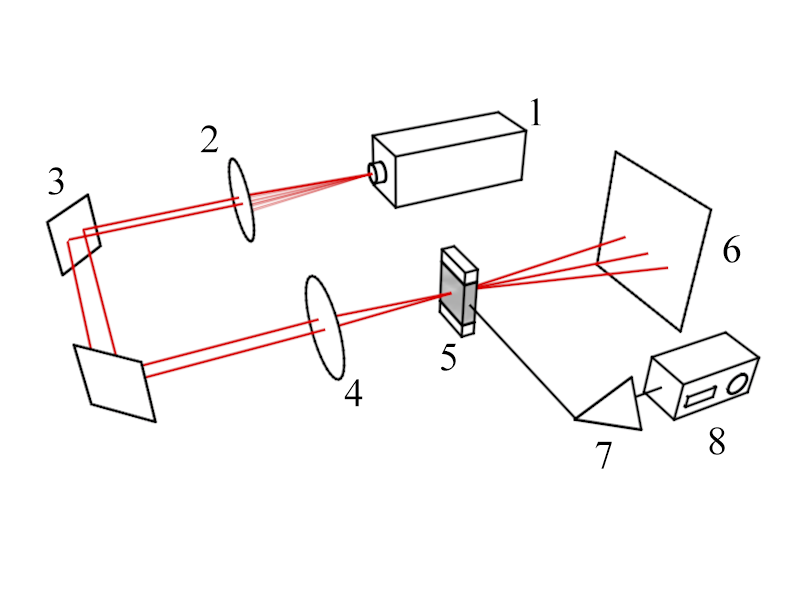
\includegraphics[width=\linewidth]{tegninger/tegning1.png}
    \caption{Opstilling til delforsøg 1.}
    \label{fig:opstilling1}
\end{figure}

\subsubsection{Dataopsamling}\label{dataopsamling1}
Først sørges for at laseren rammer AOM'ens indgang. Herefter finjusteres AOM'ens position og vinkel, således at intensiteten af førsteorden er maksimeret. Til at måle intensiteten bruges et powermeter. Nu måles afstanden mellem nulte og første orden på skærmen (pkt. 6 \cref{fig:opstilling1}) ved at lade frekvensen fra frekvensgeneratoren varierere.
Til sidst måles intensiteten af strålen ved første orden som funktion af frekvensgeneratorens effekt-output.

\subsection{Delforsøg 2}\label{dataopsamling2}
Til forskel fra delforsøg 1, placeres en switch ved pkt. $9$, i mellem frekvensgeneratoren og forstærkeren på \cref{fig:opstilling2}. Switchen er også tilkoblet et oscilloskop med indbygget frekvensgenerator. Dette tilkobles en $\SI{50}{\ohm}$ resistor for at simulere tilstedeværelsen af AOM'en. Skærmen ved pkt $6$ er brugt til at afskærme den ene stråle, hvorimod den anden stråle detekteres af en fotodetektor i pkt. $10$. Der bruges en linse til at fokusere strålen på detektoren. Herudover bruges et oscilloskop til at logge spændingen.

\begin{figure}[H]
    \centering
    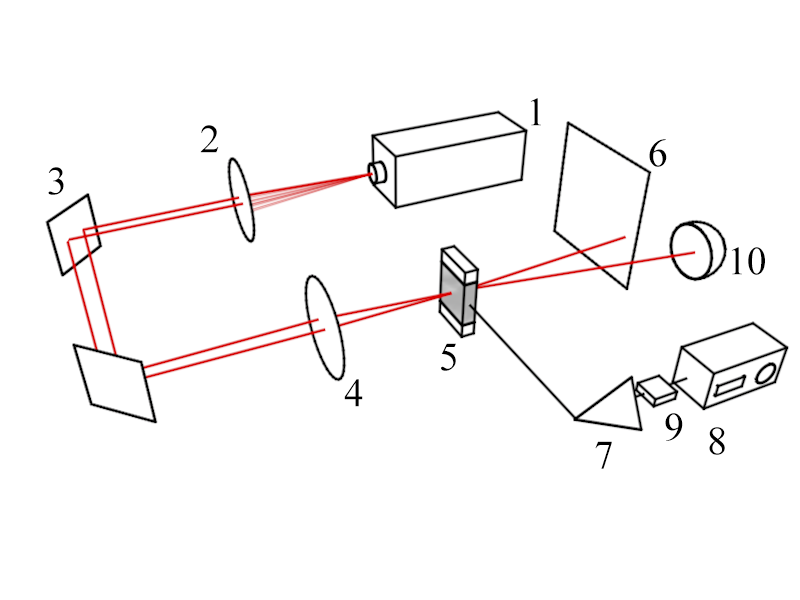
\includegraphics[width=\linewidth]{tegninger/tegning2.png}
    \caption{Opstilling til delforsøg 2.}
    \label{fig:opstilling2}
\end{figure}

\subsubsection{Dataopsamling}
I oscilloskopet er der indbygget en frekvensgenerator som sender et signal over til switch'en som har til formål at skifte signalet til et on/off signal. Først holdes AOM'en udenfor dette kredsløb så hastigheden af signalskiftet kan noteres. Hertil skrues op for frekvensen og den dertil effekt det har på switchen  som gerne skulle følge med observeres. Når dette er udført, er vi sikre på, at vi kan sende et signal som er hurtigt nok til at skifte signalet til AOM'en meget hurtigt, hvorfor vi slutter AOM'en til kredsløbet igen.

Nu ønskes der at bestemme strålens waist $w_0$. Først skal det sikres, at laserstrålen er gaussisk. Dette gøres ved at måle intensiteten som funktion af hvor meget af strålen der blokeres. I praksis gøres dette ved at tage et barberblad på en millimeter-skrue, og køre den ind foran strålen i fokallængden fra linsen. Imens dette gøres måles intensiteten af laserstrålen med en powermeter. Data tjekkes til at tilhøre en gaussisk stråle. Da dette gælder kan man finde waist, ved at tage forskellen i længden mellem de to punkter hvor laserstrålen blokeres, således at  intensiteten formindskes med $16$ og $84$ \%.
\\ Nu sættes AOM'en ind i det punkt hvor der målt waist ($z=0$). Idet switchen er sat op, kan lydbølgen tændes og slukkes hurtigt i AOM'en og den tid det tager lydbølgen at bevæge sig over laserstrålens bredde kan måles. Her er brugt en fotodetektor sat ved første orden (pkt. $10$ \cref{fig:opstilling2}. Dette gentages i forskellige bredder af laserstrålen, altså ved at sætte linser med forskellige fokallængder ind. I praksis anvende oscilloskopets cursor mode, på et datasæt hvor falltime noteres, som vist i  \cref{fig:oscillo}.

\begin{figure}[H]
    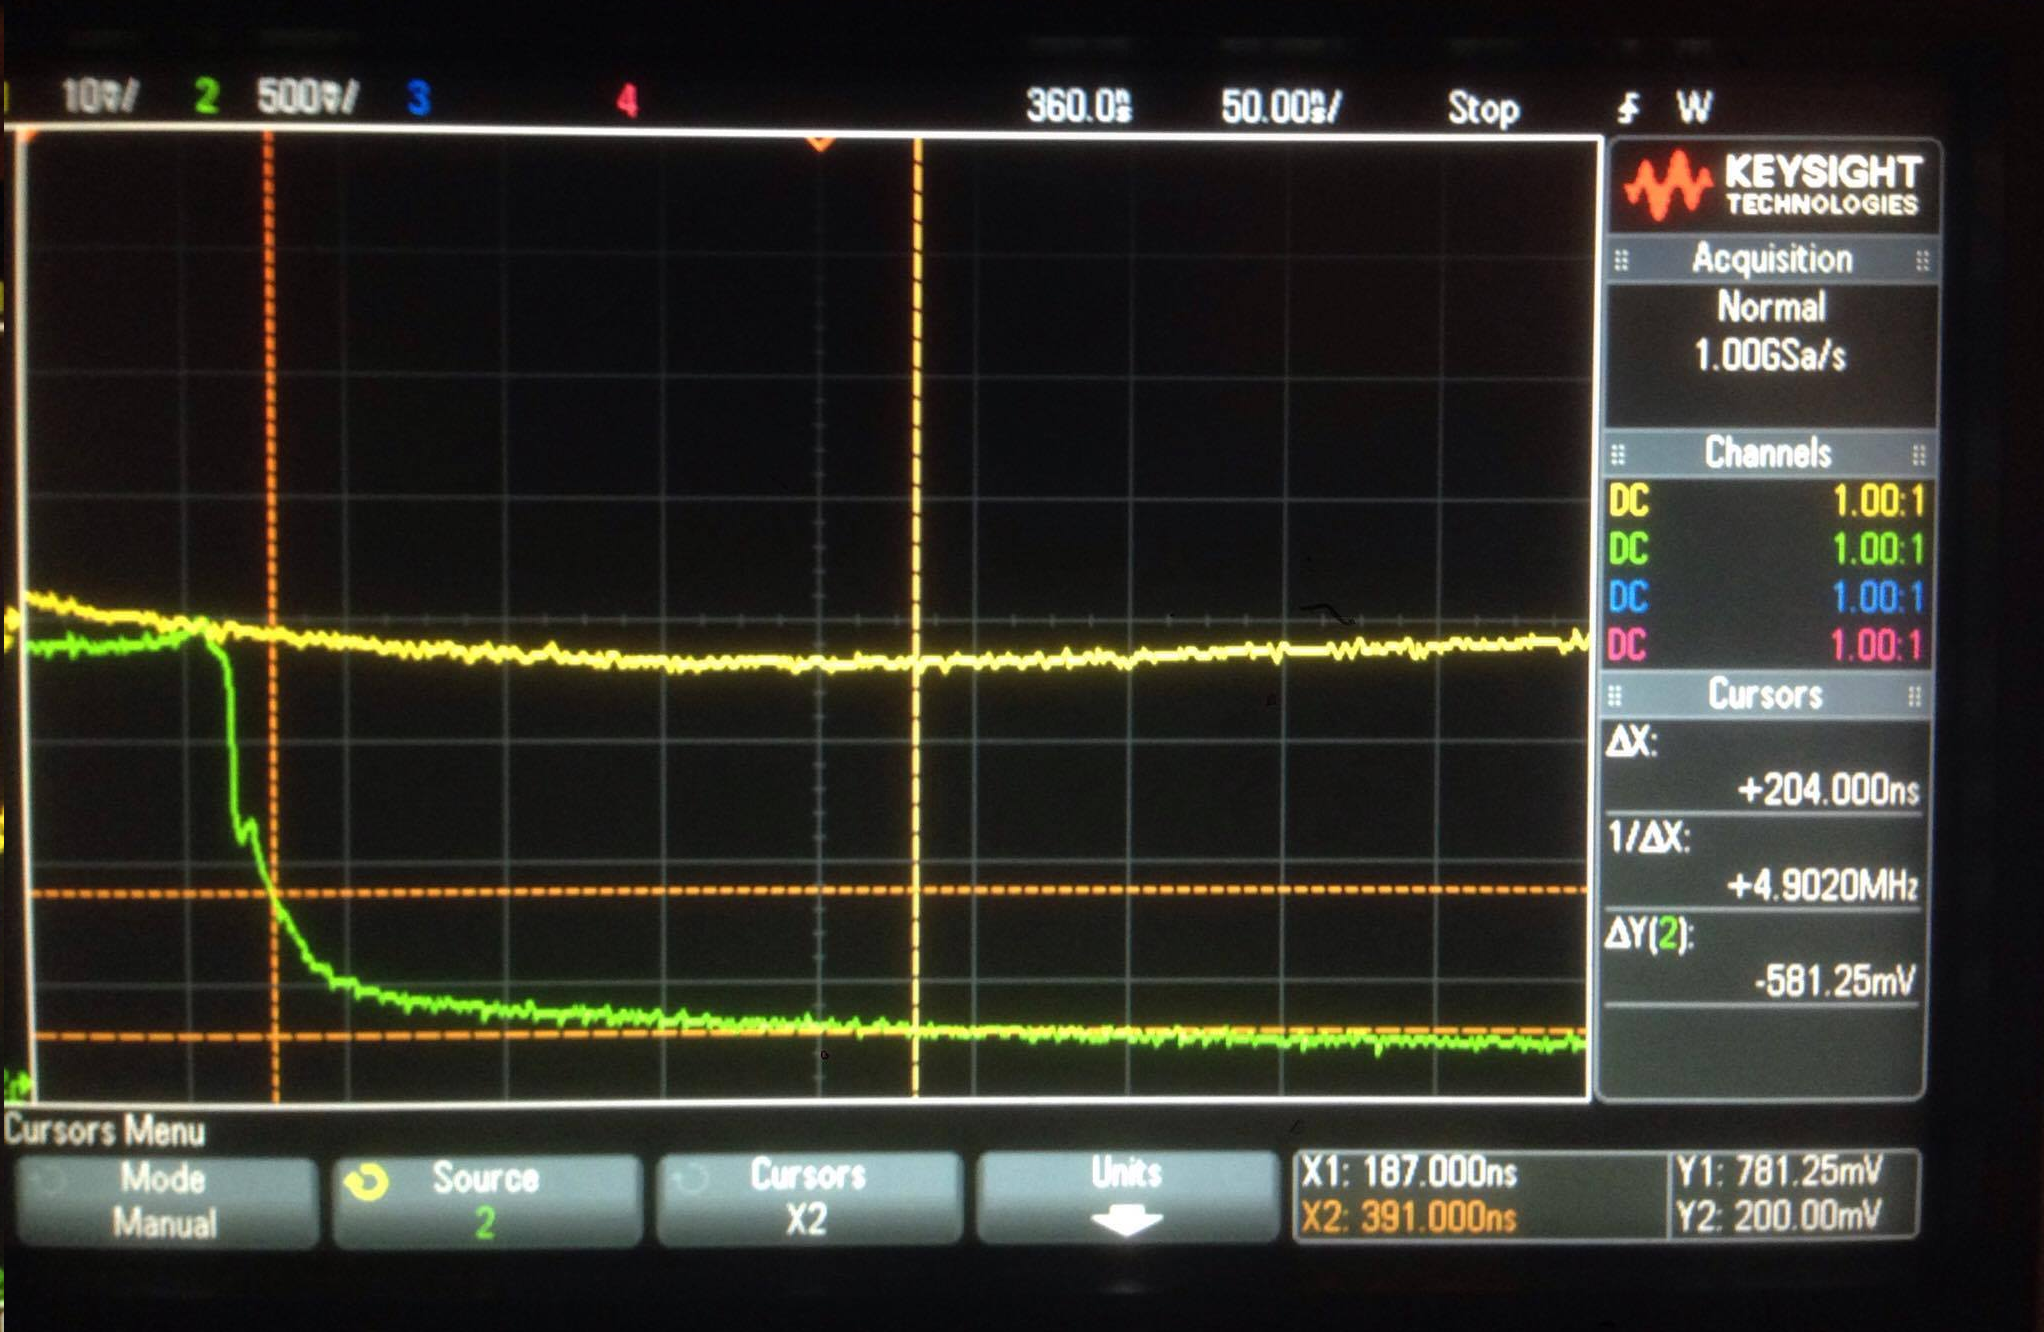
\includegraphics[width=\linewidth]{tegninger/osciolo.png}
    \caption{}
    \label{fig:oscillo}
\end{figure}

\end{document}
